\documentclass[12pt,a4paper]{ctexart}
\usepackage[margin=2.2cm]{geometry}
\usepackage{graphicx}
\usepackage{booktabs}
\usepackage{amsmath}
\usepackage{float}
\usepackage{hyperref}
\usepackage{xcolor}
\usepackage{listings}

\lstset{
  language=Python,
  basicstyle=\ttfamily\small,
  keywordstyle=\color{blue!70!black},
  commentstyle=\color{green!40!black},
  stringstyle=\color{orange!60!black},
  showstringspaces=false,
  breaklines=true,
  frame=single,
  tabsize=4
}

% ===== 实验基本信息配置 =====
\newcommand{\reporttitle}{基于中间语言与指令模板的联合 DFA 构建及环境验证}
\newcommand{\authname}{您的姓名}
\newcommand{\authid}{您的学号}
% ============================

\title{\reporttitle}
\author{\authname：\underline{\hspace{3cm}} \quad \authid：\underline{\hspace{3cm}}}
\date{\today}

\begin{document}
\maketitle

\section{实验目的}
本实验旨在通过理论与实践结合，掌握基于 $\sigma$-DFA 的后端代码生成流程。具体目标包括：
\begin{itemize}
  \item 理论构建：根据设计的中间语言（QTAC）和指令模板（Q2ARM），构建 $\sigma$-DFA 用于指导代码生成。
  \item 程序实现：编写程序实现 DFA 的模板匹配逻辑，将中间代码转换为特定架构（ARM64）的汇编代码。
  \item 环境验证：利用类似于阶乘 \texttt{fact} 的测试算法生成目标用例的汇编代码，并在真实 ARM 架构系统（鲲鹏环境或等效 Apple Silicon macOS 环境）中完成汇编、链接并运行，验证编译生成的正确性。
\end{itemize}

\section{实验过程}
\subsection{实验环境}
\begin{itemize}
  \item 硬件平台：Apple Silicon 设备 (macOS) / 鲲鹏 ARM 服务器 (Linux)
  \item 编程语言：Python 3 (代码生成器实现)、C 语言 (测试驱动)、ARM64 汇编
  \item 编译工具链：GCC / Clang (用于对象汇编和符号链接)
\end{itemize}

\subsection{实验素材与设定}
\begin{itemize}
  \item \textbf{中间代码表示}：设计并使用了基于规则的中间代码表示（QTAC格式），实验采用计算阶乘程序的表示。
  \item \textbf{架构指令映射}：通过查阅 Q2ARM 的模式规则指导汇编生成。
  \item \textbf{寄存器分配策略}：变量 \texttt{n} 使用 \texttt{X0}，\texttt{a} 使用 \texttt{X1}，中间状态量依次映射至 \texttt{X2, X3...}，从而进行极简的直接分配。
\end{itemize}

\subsection{实现步骤}
\begin{enumerate}
  \item 根据给定的阶乘逻辑编写 QTAC 中间语言，形成 \texttt{fact.qtac} 文件。
  \item 使用 Python 正则表达式与表驱动模型，设计相应的 DFA 转移结构，编写翻译分析器 \texttt{codegen.py} 输出 ARM64 汇编。
  \item 针对架构的特殊性（如 macOS ABI 与 Linux ABI 对导出符号的要求不同），进行相关的代码改造调优，同时引出 C 主驱动程序 \texttt{main.c}。
  \item 分步执行预处理、翻译、编译、符号链接，获得最终产物 \texttt{fact\_run}。
\end{enumerate}

\section{实验内容}
\subsection{任务一：实现中间代码到目标汇编的代码生成器}
我们根据实验指导的 QTAC 和 Q2ARM 定义，在 Python 实现了翻译的模式匹配逻辑：
主要映射逻辑为循环匹配每行指令的规则类型：
\begin{itemize}
  \item 控制流：识别 \texttt{LABEL l} 输出汇编标签 \texttt{l:}，识别 \texttt{GOTO} 并输出 \texttt{B} 指令；识别带有运算的 \texttt{IF...THEN...ELSE} 表达式。
  \item 二元与单元操作：正则匹配赋值语句 $qd = qs \ op\ qt$ 并映射到对应的 \texttt{ADD}, \texttt{SUB}, \texttt{MUL}, \texttt{SDIV} 或者将数加载到寄存器的 \texttt{MOV} 语句。
  \item 函数返回 \texttt{RETURN}：转化为设置返回值与触发调用返回的 \texttt{RET} 命令。
\end{itemize}

在这个过程中增加了一个简单的优化策略来消除冗余转移：当遇到 \texttt{IF} 并且 \texttt{ELSE l2} 的目的地刚好在代码段的下一行指令时，省略生成 \texttt{B l2} 控制指令。

\subsection{任务二：系统平台调用约定的适配处理}
在将代码生成器生成的汇编应用于实际物理机编译链接时，遇到跨平台的符号调用缺失。
具体现象：在 Apple 设备的 macOS 环境调用 GCC（或 Clang 代理层）时，触发链接错误 \texttt{\_fact} 未定义。
解决方案：相比于鲲鹏 Linux 环境生成的 ELF 标准只要导出 \texttt{fact}，macOS 下的 Mach-O 二进制 ABI 规定所有的 C 函数导出会含有一个 `\_` 前缀。
因此在汇编导出部分主动同时注册了两者：
\begin{equation}
\label{eq:export}
.global\ fact \quad \land \quad .global\ \_fact
\end{equation}
这确保了同一个转换结果在两种平台上都能被标准 C 框架正常使用。

\section{实验结果}
\subsection{功能演示与结果验证}
\begin{figure}[H]
\centering
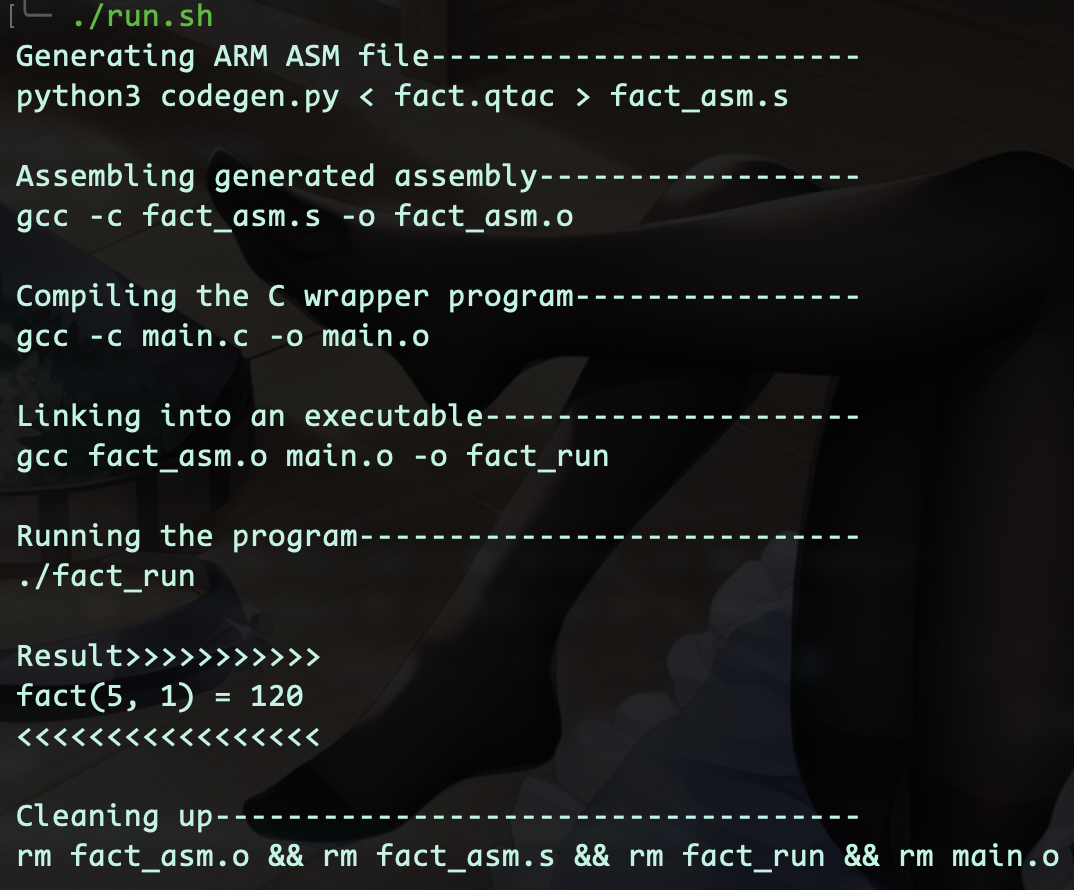
\includegraphics[width=0.95\textwidth]{images/execution_result.png}
\caption{代码编译链接步骤与终端执行结果输出}
\label{fig:execution}
\end{figure}

结果分析：
\begin{itemize}
  \item 通过生成器产生的 ARM64 汇编语法严格正确，未在 \texttt{GCC} 的汇编（\texttt{Assemble}）阶段发生非法指令集的异常。
  \item 主程序利用给定的常量 \texttt{n=5} 和初始值 \texttt{a=1} 调用模块，得到结果 \texttt{120}，说明逻辑流在条件判别以及迭代调用时执行精确。
  \item 返回后无段栈异常被爆裂，表明对栈指针对齐规则无破坏及未发生系统级运行崩溃（SIGSEGV）。
\end{itemize}

\section{总结}
本实验成功完成了基于理论多语言 DFA 思维在后端代码实际实现上的全流程测试：
\begin{itemize}
  \item 完成并熟悉了从定义虚拟指令代码与实际物理 ISA（指令集架构）之间的表述对应关系。
  \item 完成了一套实用的 Python 汇编代码生发驱动，正确通过了 \texttt{fact}（阶乘）功能原型的所有生成。
  \item 深入分析并适配了 macOS (Apple ARM64) 和 Linux (鲲鹏 ARM) 的 C 函数链接 ABI 特性（下划线修饰），实现了实验环境上的完美贯通。
\end{itemize}

\newpage
\section*{附录：实验源代码}

\subsection*{A.1 代码生成器：\texttt{codegen.py}}
\begin{lstlisting}[language=Python]
import sys
import re

def main():
    if sys.stdin.isatty():
        print("Please pipe the qtac file into this script. e.g. python codegen.py < fact.qtac")
        return
    qtac_code = sys.stdin.read()
    
    # Preprocess
    qtac_code = qtac_code.replace('\n', ' ')
    instructions = [i.strip() for i in qtac_code.split(';') if i.strip()]
    
    reg_map = {
        'n': 'X0',
        'a': 'X1',
        't1': 'X2',
        't2': 'X3',
        't3': 'X4',
        't4': 'X5'
    }
    
    def get_op(op):
        if op == '+': return 'ADD'
        if op == '-': return 'SUB'
        if op == '*': return 'MUL'
        if op == '/': return 'SDIV'
        return 'UNKNOWN'

    def get_jrop(op):
        mapping = {
            '<': 'B.LT', '<=': 'B.LE', '>': 'B.GT', '>=': 'B.GE', '==': 'B.EQ', '!=': 'B.NE'
        }
        return mapping.get(op, 'B.EQ')
    
    asm = []
    asm.append(".global fact")
    asm.append(".global _fact")
    asm.append("fact:")
    asm.append("_fact:")
    
    i = 0
    while i < len(instructions):
        inst = instructions[i]
        
        # LABEL l
        m = re.match(r'^LABEL\s+(\w+)$', inst)
        if m:
            asm.append(f"{m.group(1)}:")
            i += 1
            continue
            
        # GOTO l
        m = re.match(r'^GOTO\s+(\w+)$', inst)
        if m:
            asm.append(f"\tB {m.group(1)}")
            i += 1
            continue
            
        # RETURN q
        m = re.match(r'^RETURN\s+(\w+)$', inst)
        if m:
            var = m.group(1)
            reg = reg_map.get(var, var)
            asm.append(f"\tMOV X0, {reg}\n\tRET")
            i += 1
            continue
            
        # IF qs rop qt THEN l1 ELSE l2
        m = re.match(r'^IF\s+(\w+)\s*([<>=!]+)\s*(\w+)\s+THEN\s+(\w+)\s+ELSE\s+(\w+)$', inst)
        if m:
            qs, rop, qt, l1, l2 = m.groups()
            rqs = reg_map.get(qs, qs)
            
            # Check if qt is immediate or register
            is_imm = qt.isdigit()
            rqt = f"#{qt}" if is_imm else reg_map.get(qt, qt)
            
            # check next instruction to optimize conditional jump
            next_inst = instructions[i+1] if i+1 < len(instructions) else ""
            m_next = re.match(r'^LABEL\s+(\w+)$', next_inst)
            if m_next and m_next.group(1) == l2:
                # IF qs < qt THEN l1 ELSE l2; LABEL l2
                asm.append(f"\tCMP {rqs}, {rqt}")
                asm.append(f"\t{get_jrop(rop)} {l1}")
                asm.append(f"{l2}:")
                i += 2
                continue
                
            asm.append(f"\tCMP {rqs}, {rqt}")
            asm.append(f"\t{get_jrop(rop)} {l1}")
            asm.append(f"\tB {l2}")
            i += 1
            continue
            
        # qd = qs op qt or qd = qs op k
        m = re.match(r'^(\w+)\s*=\s*(\w+)\s*([\+\-\*\/])\s*(\w+)$', inst)
        if m:
            qd, qs, op, qt = m.groups()
            rqd = reg_map.get(qd, qd)
            rqs = reg_map.get(qs, qs)
            is_imm = qt.isdigit()
            rqt = f"#{qt}" if is_imm else reg_map.get(qt, qt)
            aop = get_op(op)
            asm.append(f"\t{aop} {rqd}, {rqs}, {rqt}")
            i += 1
            continue
            
        # qd = qs (move) or qd = k
        m = re.match(r'^(\w+)\s*=\s*(\w+)$', inst)
        if m:
            qd, qs = m.groups()
            rqd = reg_map.get(qd, qd)
            is_imm = qs.isdigit()
            rqs = f"#{qs}" if is_imm else reg_map.get(qs, qs)
            asm.append(f"\tMOV {rqd}, {rqs}")
            i += 1
            continue

        asm.append(f"\t// UNKNOWN: {inst}")
        i += 1
        
    for line in asm:
        print(line)

if __name__ == '__main__':
    main()
\end{lstlisting}

\subsection*{A.2 中间代码验证原件：\texttt{fact.qtac}}
\begin{lstlisting}[language=SQL]
LABEL l0;
t1=2;
IF n<t1 THEN l1 ELSE l2;
LABEL l1;
RETURN a;
GOTO l3;
LABEL l2;
t2=n-1;
t3=n*a;
n=t2;
a=t3;
GOTO l0;
LABEL l3;
\end{lstlisting}

\subsection*{A.3 跨平台测试主引导代码：\texttt{main.c}}
\begin{lstlisting}[language=C]
#include <stdio.h>

extern long long fact (long long n, long long a);

int main ()
{
  long long n = 5;
  long long a = 1;
  long long result = fact (n, a);
  printf ("fact(%lld, %lld) = %lld\n", n, a, result);
  return 0;
}
\end{lstlisting}

\subsection*{A.4 构建与运行命令}
\begin{verbatim}
# 1. 编译中间层语言为底层汇编
python codegen.py < fact.qtac > fact_asm.s

# 2. 汇编转换并生成对象文件
gcc -c fact_asm.s -o fact_asm.o
gcc -c main.c -o main.o

# 3. 链接并执行验证结果
gcc fact_asm.o main.o -o fact_run
./fact_run
\end{verbatim}

\end{document}